\chapter{Expérimentations et Résultats}

En raison des difficultés d'accès aux données spectrales \acrshort{MS} et \acrshort{RMN} communes sur des molécules ainsi que de l'accès au code source de GNPS, nous avons mené les expérimentations sur l'étape de construction des clusters de l'approche de type Bagging.

\section{Jeu de données}

    Nous avons mené les expérimentations sur la dataset MSRC-V1 d'images qui contient 210 objets pour 7 classes.
    Les 7 classes correspondent à des arbres, des bâtiments, des avions, des visages, des voitures, des bœufs et des bicyclettes.
    Ce dataset contient 4 vues qui correspondent à des caractéristiques extraites de ces images.

\section{Métriques d'évaluation}

 	Comme métrique de performances, nous avons utilisé:
	\begin{itemize}
  	  \item Exactitude (ACC) : qui permet de mesurer à quel point les clusters construits ressemblent à ceux de la réalité, en évaluant la correspondance maximale entre elles.
  	  \begin{equation}
  		  ACC(X,Y) = \max_{alloc \in P} \frac{1}{n} \sum_{i=1}^{n} 1(alloc(Y_i) = X_i)
  	  \end{equation}
  	  avec $n$ le nombre d'observations, $P$ étant l'ensemble des allocations possibles des clusters  du regroupement $X$ aux clusters du regroupement $Y$.
      
  	  \item Information mutuelle normalisée (\acrshort{NMI}) : qui permet de mesurer la quantité d'informations partagées entre les clusters construits et les clusters réels.

  	  \begin{equation}
     	   \text{NMI}(X,Y) = \frac{ \sum_{k=1}^{K^{(X)}} \sum_{k'=1}^{K^{(Y)}} n_{k,k'} \log\left( \frac{N \times n_{k,k'}}{ n_k^{(X)} n_{k'}^{(Y)} } \right) }{  \sqrt{ \left( \sum_{k=1}^{K^{(X)}} n_k^{(X)}\log( \frac{n_k^{(X)}}{N} )  \right) \left( \sum_{k'=1}^{K^{(Y)}} n_{k'}^{(Y)} \log( \frac{n_{k'}^{(Y)}}{N} )  \right)  } }
		   	\label{equa:enss2}
  	  \end{equation}
  	  avec $n_k^{(X)}$ étant le nombre d'observations contenues dans le cluster $k$ du regroupement $X$, $n_{k'}^{(Y)}$ étant le nombre d'observations contenues dans le cluster $k'$ du regroupement $Y$, $n_{k,k'}$ étant le nombre d'observations étant dans les clusters $k$ et $k'$, $K^{(X)}$ étant le nombre de clusters du regroupement $X$, $K^{(Y)}$ étant le nombre de clusters du regroupement $Y$.
      
  	  \item Pureté (PUR) : qui permet de mesurer le degré d'homogénéité des clusters construits par rapport aux groupes réels, en pénalisant les potentiels bruits dans ces clusters construits.

  	  \begin{equation}
  		  PUR(X,Y) = \frac{ \sum_{ y \in Y'} \left( \max_{x \in X'} card(\{ i| X_i = x, Y_i = y, i \in 1..n \})\right)}{n}
  	  \end{equation}
  	  avec $X'$ et $Y'$ étant les ensembles des clusters des regroupements $X$ et $Y$ respectivement
	\end{itemize}

 \section{Protocole expérimentale}

    Pour mener à bien les expérimentations, nous avons utilisé un ordinateur portable ayant les caractéristiques suivantes:
	\begin{itemize}
  	  \item 8 CPUs (2.4Ghz de fréquence chacun)
  	  \item 12 Go de mémoire
	\end{itemize}

    Nous avons utilisé le langage de programmation {python} avec comme librairies utiles:
    \begin{itemize}
   	 \item numpy: pour réaliser les calculs vectoriels
   	 \item qpsolvers: pour résoudre les problèmes d'optimisation quadratiques liés à MCLES
   	 \item ClusterEnsembles : pour utiliser les algorithmes d'ensemble de clustering
    \end{itemize}

    Nous avons également exécuté chaque modèle sujet à l'expérimentation 10 fois de suite. Ce qui nous a conduit à calculer la moyenne et l'écart des performances obtenues pour avoir les performances définitives.
    
\section{Résultats}

	Pour observer le comportement des performances de la méthode proposée selon le pourcentage d'observations utilisé pour les échantillons (\textbf{\textit{p}}) et le nombre de weak-learners utilisés (\textbf{\textit{nw}}), nous avons fixé une grille d'exploration avec le pourcentage \textbf{\textit{p}} allant de 50\% à 90\% avec des pas de 5\% et le nombre \textbf{\textit{nw}} allant de 40 à 160 avec des pas 40.

    Avec MCLES en weak-learner, on remarque que le graphe de l'exactitude (voir la Figure \ref{fig:bagmcles_acc_3d}) par rapport à tous les paramètres, présente une courbe parabolique dépendante principalement de la taille des échantillons \textit{p}, où la zone de meilleures valeurs est décrite par des valeurs de \textit{p} comprises entre 65\% à 80\%, et des valeurs de \textit{nw} de plus de 100.
    On y observe une légère hausse d'exactitude pour \textit{p} allant de 50\% à 80\%, puis d'une forte baisse pour \textit{p} à plus de 80\% quelque soit les valeurs de \textit{nw} (Voir également la Figure \ref{fig:bagmcles_acc_p}).
    On remarque plus précisément sur la Figure \ref{fig:bagmcles_acc_nw} qu'on a une tendance de légère hausse par rapport à \textit{nw} avec de meilleures valeurs quand \textit{p} est compris entre 60\% et 80\%.
    Tout ceci nous permet d'affirmer que l'exactitude du modèle dépend plus fortement de la taille des échantillons que du nombre de weak-learners utilisés.

    \begin{figure}
  		 \centering
  		 \begin{subfigure}{0.3\linewidth}
  			 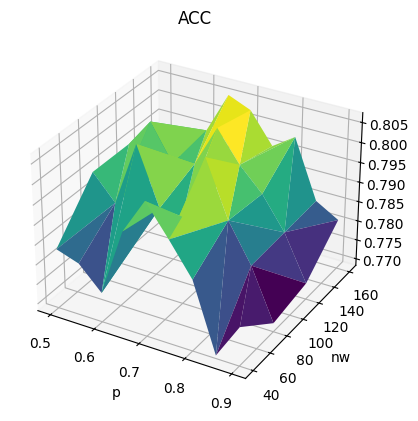
\includegraphics[width=\linewidth]{Images/ACC_mcles.png}
  			 \caption{Suivant tous les paramètres}
  			 \label{fig:bagmcles_acc_3d}
  			 \end{subfigure}
    	\begin{subfigure}{0.3\linewidth}
  	   	  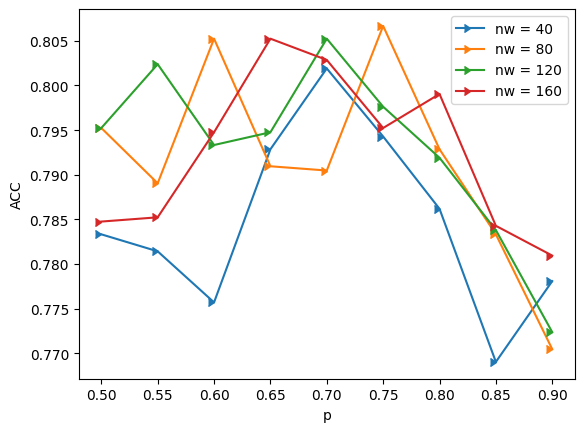
\includegraphics[width=\linewidth]{Images/ACC_mcles_p.png}
  			 \caption{Suivant la taille des échantillons}
  			 \label{fig:bagmcles_acc_p}
  		 \end{subfigure}
    	\begin{subfigure}{0.3\linewidth}
  			 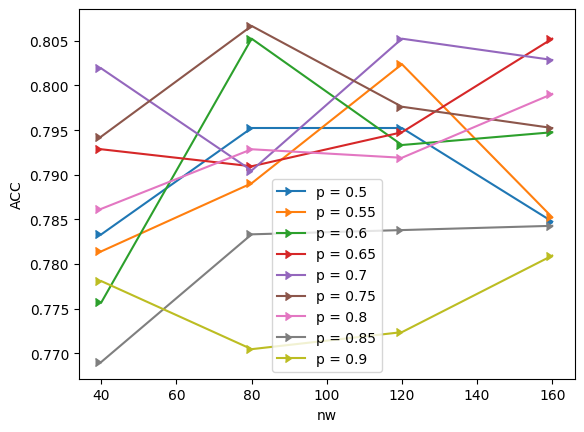
\includegraphics[width=\linewidth]{Images/ACC_mcles_nw.png}
  			 \caption{Suivant le nombre de weak-learners}
  	   	  \label{fig:bagmcles_acc_nw}
  		 \end{subfigure}
  		 \caption{Graphes de l'exactitude pour l'approche de type Bagging avec MCLES}
  		 \label{fig:bagmcles_acc}
	\end{figure}

    Pour le graphe de l'information mutuelle normalisée présente sur la Figure \ref{fig:bagmcles_nmi_3d}, on remarque que plus la taille \textit{p} des échantillons utilisés augmente, plus l'information mutuelle normalisée augmente aussi.
    De plus, l'augmentation de \textit{nw} conduit également à une légère hausse de cette même information mutuelle. On retrouve cette augmentation par rapport à \textit{p} sur la Figure \ref{fig:bagmcles_nmi_p} quelque soit le nombre \textit{nw} de weak-learners utilisés.
    On remarque également comme pour l'exactitude une légère hausse de l'information mutuelle normalisée par rapport à \textit{nw} (voir la Figure \ref{fig:bagmcles_nmi_nw}), avec de meilleures valeurs quand \textit{p} est compris entre 70\% et 80\%.
    Ce qui nous montre qu'on a une corrélation positive entre l'information mutuelle et les deux paramètres, qui est plus forte avec la taille des échantillons.
    
    \begin{figure}
  		 \centering
  		 \begin{subfigure}{0.3\linewidth}
  			 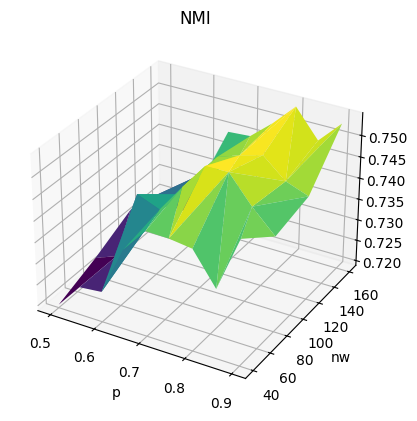
\includegraphics[width=\linewidth]{Images/NMI_mcles.png}
  			 \caption{Suivant tous les paramètres}
  			 \label{fig:bagmcles_nmi_3d}
  			 \end{subfigure}
    	\begin{subfigure}{0.3\linewidth}
  	   	  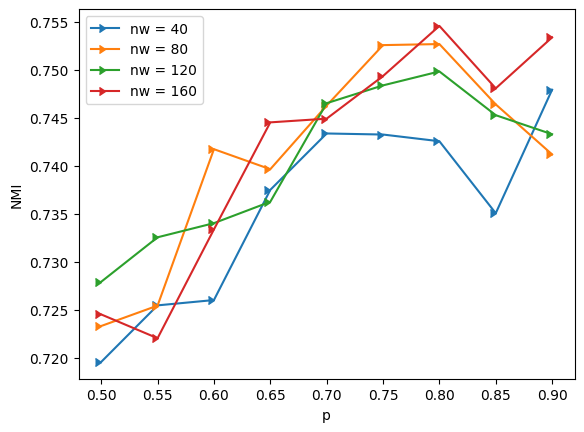
\includegraphics[width=\linewidth]{Images/NMI_mcles_p.png}
  			 \caption{Suivant la taille des échantillons}
  			 \label{fig:bagmcles_nmi_p}
  		 \end{subfigure}
    	\begin{subfigure}{0.3\linewidth}
  			 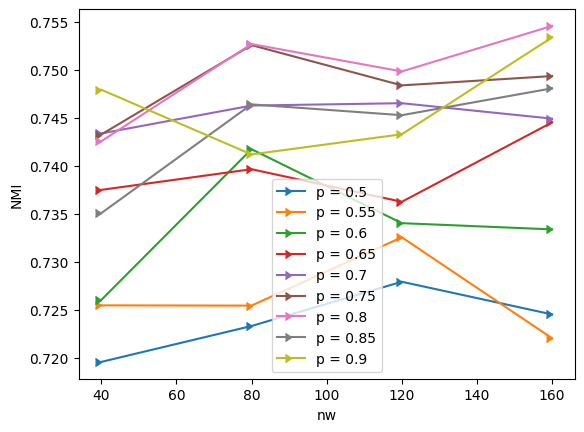
\includegraphics[width=\linewidth]{Images/NMI_mcles_nw.png}
  			 \caption{Suivant le nombre de weak-learners}
  	   	  \label{fig:bagmcles_nmi_nw}
  		 \end{subfigure}
  		 \caption{Graphes de l'information mutuelle normalisée pour la méthode de type Bagging avec MCLES}
  		 \label{fig:bagmcles_acc}
	\end{figure}

    Pour la pureté, on observe sur son graphe de Figure \ref{fig:bagmcles_pur_3d} une courbe parabolique dépendant principalement de la taille des échantillons \textit{p} comme pour le cas de l'exactitude, avec la zone de meilleures valeurs étant décrite par des valeurs de \textit{p} comprises entre 65\% à 75\%, et des valeurs du nombre \textit{nw} de weak-learners de plus de 80.
    On revoit sur la Figure \ref{fig:bagmcles_pur_p} la parabole du graphe précédent, où on observe plus clairement une augmentation générale de la pureté par rapport à \textit{p} de 50\% à 80\% puis d'une forte baisse de 80\% à plus, quelque soit les valeurs de \textit{nw}.
    De plus, on retrouve comme pour les autres métriques, une faible augmentation générale de la pureté par rapport à \textit{nw}, avec de meilleures valeurs quand \textit{p} est compris entre 70\% à 80\%  (voir la Figure \ref{fig:bagmcles_pur_nw}).
    De là, on remarque encore une dépendance visible de la pureté par rapport à la taille des échantillons.
    \begin{figure}
  		 \centering
  		 \begin{subfigure}{0.3\linewidth}
  			 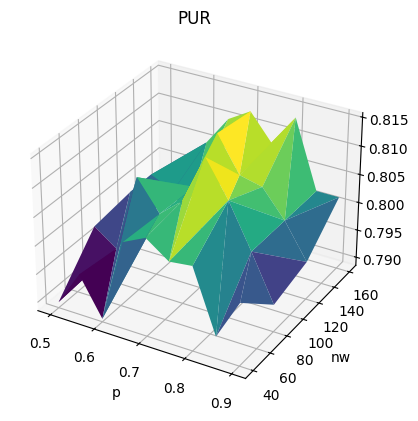
\includegraphics[width=\linewidth]{Images/PUR_mcles.png}
  			 \caption{Suivant tous les paramètres}
  			 \label{fig:bagmcles_pur_3d}
  			 \end{subfigure}
    	\begin{subfigure}{0.3\linewidth}
  	   	  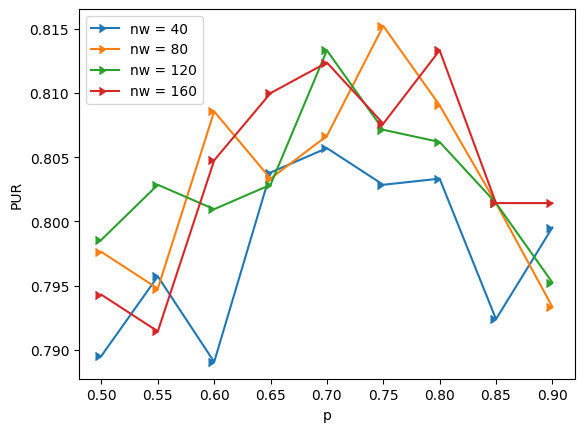
\includegraphics[width=\linewidth]{Images/PUR_mcles_p.png}
  			 \caption{Suivant la taille des échantillons}
  			 \label{fig:bagmcles_pur_p}
  		 \end{subfigure}
    	\begin{subfigure}{0.3\linewidth}
  			 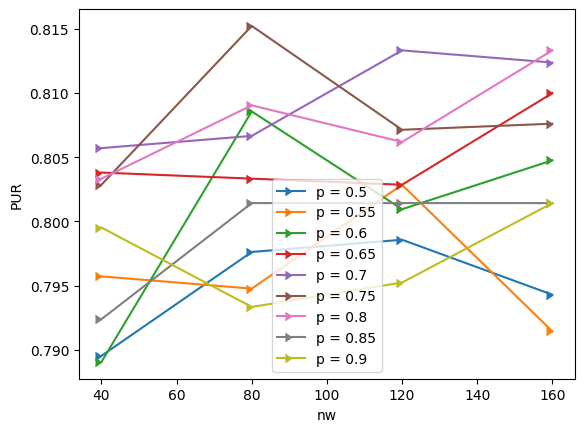
\includegraphics[width=\linewidth]{Images/PUR_mcles_nw.png}
  			 \caption{Suivant le nombre de weak-learners}
  	   	  \label{fig:bagmcles_pur_nw}
  		 \end{subfigure}
  		 \caption{Graphes de la pureté pour la méthode de type Bagging avec MCLES}
  		 \label{fig:bagmcles_acc}
	\end{figure}

    On peut donc conclure que plus on augmente la taille des échantillons, plus on augmente les informations communes entre les clusters construits et les groupes réels.
    Néanmoins elle doit être ni trop grande ni trop petite pour obtenir des clusters plus homogènes correspondant de mieux en mieux à ceux de la réalité.
    De façon générale, l'augmentation du nombre de weak-learners permet d'améliorer bien que légèrement la qualité des clusters construits.
    On retrouve ainsi qu'il est favorable d'utiliser \textbf{70\% à 80\%} des observations pour construire les échantillons et \textbf{le plus possible} de weak-learners dans le cas où on a MCLES en weak-learner. Les Tableaux \ref{table:acc_mcles}, \ref{table:nmi_mcles}, \ref{table:pur_mcles} permettent également d'appuyer nos observations.
    
	\begin{table}[h!]
  		 \caption{Tableau croisé de l'exactitude pour la méthode de type Bagging avec MCLES}
  		 \centering
  		 \begin{tabular}{lrrrr}
    	\toprule
    	nw & 40 & 80 & 120 & 160 \\
    	p &  &  &  &  \\
    	\midrule
    	50\% & 0.7833 & 0.7952 & 0.7952 & 0.7847 \\
    	55\% & 0.7814 & 0.7890 & 0.8023 & 0.7852 \\
    	60\% & 0.7757 & 0.8052 & 0.7933 & 0.7947 \\
    	65\% & 0.7928 & 0.7909 & 0.7947 & \textbf{0.8052} \\
    	70\% & \textbf{0.8019} & 0.7904 & \textbf{0.8052} & 0.8028 \\
    	75\% & 0.7942 & \textbf{0.8066} & 0.7976 & 0.7952 \\
    	80\% & 0.7861 & 0.7928 & 0.7919 & 0.7990 \\
    	85\% & 0.7690 & 0.7833 & 0.7838 & 0.7842 \\
    	90\% & 0.7780 & 0.7704 & 0.7723 & 0.7809 \\
    	\bottomrule
    	\end{tabular}
  		 \label{table:acc_mcles}
	\end{table}

	\begin{table}[h!]
  		 \caption{Tableau croisé de l'information mutuelle normalisée pour la méthode de type Bagging avec MCLES}
  		 \centering
    	\begin{tabular}{lrrrr}
    	\toprule
    	nw & 40 & 80 & 120 & 160 \\
    	p &  &  &  &  \\
    	\midrule
    	50\% & 0.7195 & 0.7233 & 0.7279 & 0.7245 \\
    	55\% & 0.7254 & 0.7254 & 0.7325 & 0.7220 \\
    	60\% & 0.7260 & 0.7417 & 0.7340 & 0.7333 \\
    	65\% & 0.7374 & 0.7396 & 0.7362 & 0.7445 \\
    	70\% & 0.7433 & 0.7462 & 0.7465 & 0.7448 \\
    	75\% & 0.7432 & 0.7525 & 0.7483 & 0.7493 \\
    	80\% & 0.7425 & \textbf{0.7526} & \textbf{0.7498} & \textbf{0.7545} \\
    	85\% & 0.7350 & 0.7463 & 0.7452 & 0.7480 \\
    	90\% & \textbf{0.7479} & 0.7411 & 0.7432 & 0.7533 \\
    	\bottomrule
    	\end{tabular}
  		 \label{table:nmi_mcles}
	\end{table}

	\begin{table}[h!]
  		 \caption{Tableau croisé de la pureté pour la méthode de type Bagging avec MCLES}
  		 \centering
    	\begin{tabular}{lrrrr}
    	\toprule
    	nw & 40 & 80 & 120 & 160 \\
    	p &  &  &  &  \\
    	\midrule
    	50\% & 0.7895 & 0.7976 & 0.7985 & 0.7942 \\
    	55\% & 0.7957 & 0.7947 & 0.8028 & 0.7914 \\
    	60\% & 0.7890 & 0.8085 & 0.8009 & 0.8047 \\
    	65\% & 0.8038 & 0.8033 & 0.8028 & 0.8100 \\
    	70\% & \textbf{0.8057} & 0.8066 & \textbf{0.8133} & 0.8123 \\
    	75\% & 0.8028 & 0.8152 & 0.8071 & 0.8076 \\
    	80\% & 0.8033 & \textbf{0.8090} & 0.8061 & \textbf{0.8133} \\
    	85\% & 0.7923 & 0.8014 & 0.8014 & 0.8014 \\
    	90\% & 0.7995 & 0.7933 & 0.7952 & 0.8014 \\
    	\bottomrule
    	\end{tabular}
  		 \label{table:pur_mcles}
	\end{table}


    Avec MVGL en weak-learner, on remarque que le graphe de l'exactitude de Figure \ref{fig:bagmvgl_acc_3d}, présente une courbe parabolique dépendante principalement de la taille \textit{p} des échantillons utilisés.
    On y trouve les meilleures valeurs d'exactitude quand \textit{p} est compris entre 50\% à 55\% et le nombre \textbf{nw} de weak-learners dépasse 120.
    Comme sur la Figure \ref{fig:bagmvgl_acc_p}, on observe également une forte baisse d'exactitude pour \textit{p} allant de 50\% à 70\%, puis d'une hausse pour \textit{p} de plus de 70\%, quel que soit le nombre \textit{nw} de weak-learner.
    On remarque une forte hausse d'exactitude par rapport à \textit{nw} quand  \textit{p} est compris entre 50\% et 55\%, mais une tendance plus légère pour des valeurs de  \textit{p} de plus de 55\% (Voir également la Figure \ref{fig:bagmvgl_acc_nw}).
    Nous pouvons donc affirmer que l'exactitude dépend plus fortement de la taille des échantillons que du nombre de weak-learners.

    \begin{figure}
        \centering
        \begin{subfigure}{0.3\linewidth}
     	   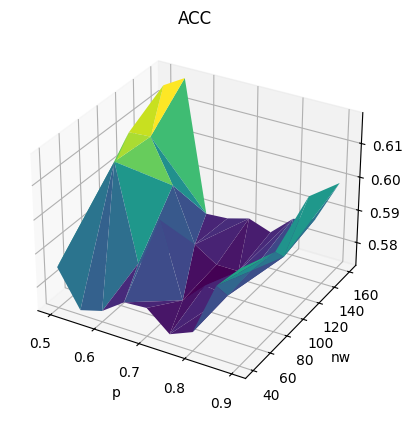
\includegraphics[width=\linewidth]{Images/ACC_mvgl.png}
     	   \caption{Suivant tous les paramètres}
     	   \label{fig:bagmvgl_acc_3d}
     	   \end{subfigure}
        \begin{subfigure}{0.3\linewidth}
     	   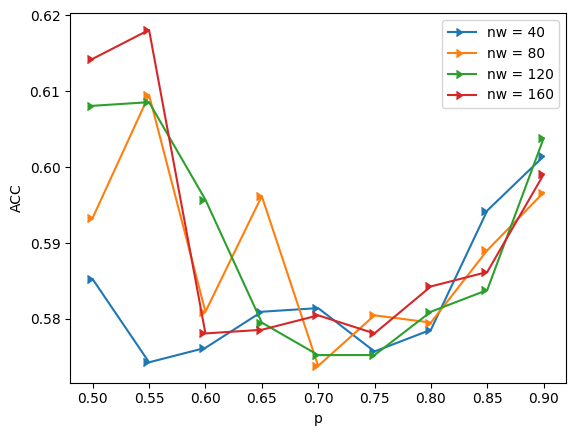
\includegraphics[width=\linewidth]{Images/ACC_mvgl_p.png}
     	   \caption{Suivant la taille des échantillons}
     	   \label{fig:bagmvgl_acc_p}
        \end{subfigure}
        \begin{subfigure}{0.3\linewidth}
     	   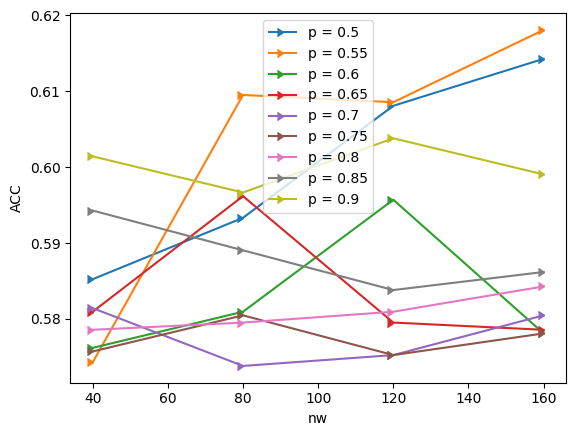
\includegraphics[width=\linewidth]{Images/ACC_mvgl_nw.png}
     	   \caption{Suivant le nombre de weak-learners}
     	   \label{fig:bagmvgl_acc_nw}
        \end{subfigure}
        \caption{Graphes de l'exactitude pour la méthode de type Bagging avec MVGL}
        \label{fig:bagmvgl_acc}
    \end{figure}

    Pour le graphe de l'information mutuelle normalisée, visible sur la Figure \ref{fig:bagmvgl_nmi_3d}, plus la taille des échantillons augmente, plus cette information mutuelle diminue.
    L'augmentation du nombre \textit{nw} de weak-learners présente une légère hausse de l'information mutuelle normalisée.
    On retrouve aussi sur la Figure \ref{fig:bagmvgl_nmi_p} cette corrélation entre \textit{p} et l'information mutuelle normalisée quelque soit les valeurs de \textit{nw}.
    On remarque également avec plus de précision sur la Figure \ref{fig:bagmvgl_nmi_nw} que l'augmentation de \textit{nw} conduit généralement à une légère hausse de l'information mutuelle, mais qui devient plus forte pour des valeurs de \textit{p} comprises entre 50\% et 55\%.
    Cela montre que l'information mutuelle dépend négativement de la taille des échantillons et positivement du nombre de weak-learners utilisés.
    
    \begin{figure}
        \centering
        \begin{subfigure}{0.3\linewidth}
     	   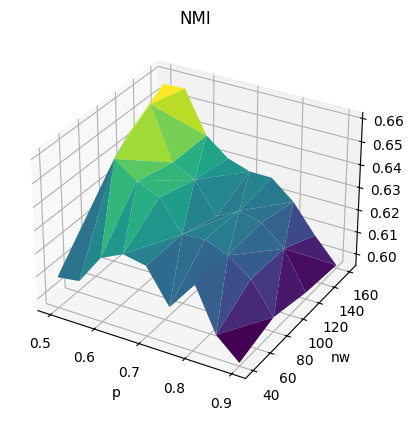
\includegraphics[width=\linewidth]{Images/NMI_mvgl.png}
     	   \caption{Suivant tous les paramètres}
     	   \label{fig:bagmvgl_nmi_3d}
     	   \end{subfigure}
 	\begin{subfigure}{0.3\linewidth}
     	   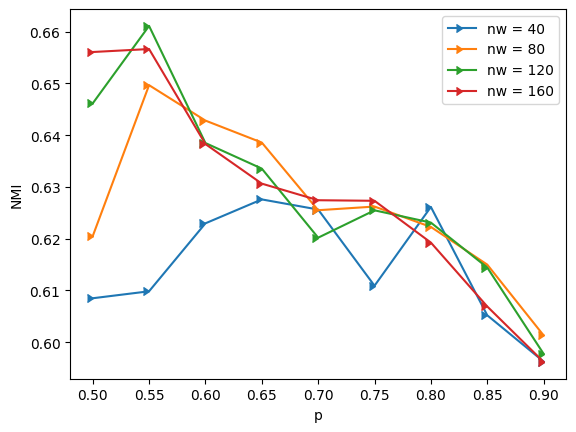
\includegraphics[width=\linewidth]{Images/NMI_mvgl_p.png}
     	   \caption{Suivant la taille des échantillons}
     	   \label{fig:bagmvgl_nmi_p}
        \end{subfigure}
 	\begin{subfigure}{0.3\linewidth}
     	   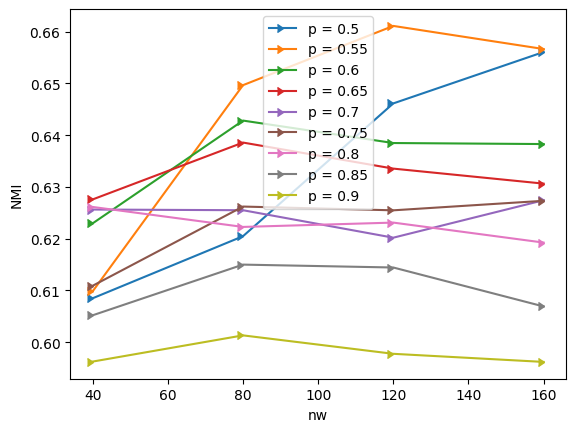
\includegraphics[width=\linewidth]{Images/NMI_mvgl_nw.png}
     	   \caption{Suivant le nombre de weak-learners}
     	   \label{fig:bagmvgl_nmi_nw}
        \end{subfigure}
        \caption{Graphes de l'information mutuelle normalisée pour la méthode de type Bagging avec MVGL}
        \label{fig:bagmvgl_acc}
    \end{figure}

    Pour la pureté, son graphe de Figure \ref{fig:bagmvgl_pur_3d} montre que plus la taille \textit{p} des échantillons augmente, plus la pureté augmente. On peut également y voir que l'augmentation du nombre \textit{nw} de weak-learners conduit à une hausse plus légère de pureté. On revoit également ces faits sur la Figure \ref{fig:bagmvgl_pur_p},où l’augmentation générale de la pureté qui devient plus forte lorsque \textit{p} est supérieur à 80\% quelque soit le nombre de weak-learners.
    On retrouve aussi sur la Figure \ref{fig:bagmcles_pur_nw} une hausse légère de performance par rapport à \textit{nw}, avec de meilleures valeurs quand \textit{p} est à plus de 85\%.
    On peut donc affirmer qu'on a une corrélation positive entre la pureté et les paramètres, qui est plus forte avec la taille des échantillons.
    
    \begin{figure}
        \centering
        \begin{subfigure}{0.3\linewidth}
     	   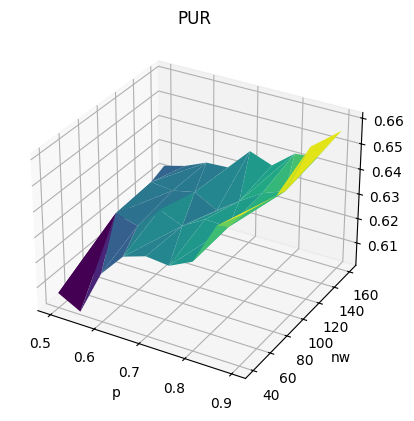
\includegraphics[width=\linewidth]{Images/PUR_mvgl.png}
     	   \caption{Suivant tous les paramètres}
     	   \label{fig:bagmvgl_pur_3d}
     	   \end{subfigure}
        \begin{subfigure}{0.3\linewidth}
     	   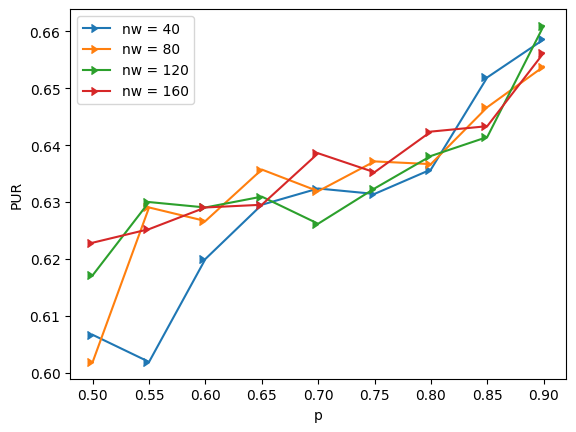
\includegraphics[width=\linewidth]{Images/PUR_mvgl_p.png}
     	   \caption{Suivant la taille des échantillons}
     	   \label{fig:bagmvgl_pur_p}
        \end{subfigure}
        \begin{subfigure}{0.3\linewidth}
     	   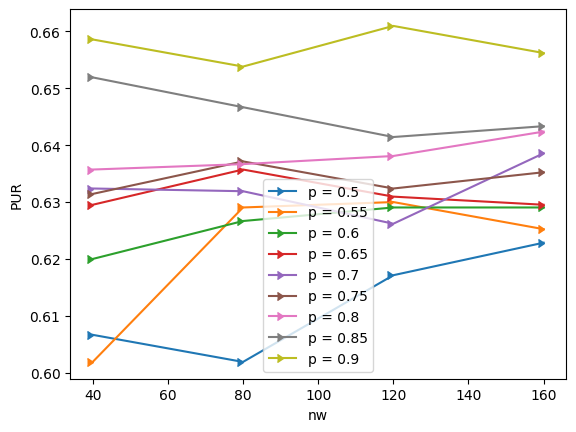
\includegraphics[width=\linewidth]{Images/PUR_mvgl_nw.png}
     	   \caption{Suivant le nombre de weak-learners}
     	   \label{fig:bagmvgl_pur_nw}
        \end{subfigure}
        \caption{Graphes de la pureté pour la méthode de type Bagging avec MVGL}
        \label{fig:bagmvgl_acc}
    \end{figure}

    
    Nous pouvons ainsi conclure que plus on augmente la taille des échantillons, plus on a tendance à avoir des clusters plus homogènes, mais qui correspondent moins aux groupes réels avec une réduction de la quantité d’informations communes.
    Ce qui nous amène à voir que nous avons une corrélation négative entre la pureté et l'information mutuelle normalisée.
    On retrouve ainsi grâce à ces observations qu'il est favorable d'utiliser \textit{50\% à 55\%} des observations pour construire des échantillons et le plus possible de weak-learners dans le cas où MVGL est en weak-learner. Les Tableaux de performances \ref{table:acc_mvgl}, \ref{table:nmi_mvgl} et \ref{table:pur_mvgl} permettent d'appuyer nos observations.

	\begin{table}[h!]
  		 \caption{Tableau croisé de l'exactitude pour la méthode de type Bagging avec MVGL}
  		 \centering
  		 \begin{tabular}{lrrrr}
    	\toprule
    	nw & 40 & 80 & 120 & 160 \\
    	p &  &  &  &  \\
    	\midrule
    	50\% & 0.5852 & 0.5933 & 0.6080 & 0.6142 \\
    	55\% & 0.5742 & \textbf{0.6095} & \textbf{0.6085} & \textbf{0.6180} \\
    	60\% & 0.5761 & 0.5809 & 0.5957 & 0.5780 \\
    	65\% & 0.5809 & 0.5961 & 0.5795 & 0.5785 \\
    	70\% & 0.5814 & 0.5738 & 0.5752 & 0.5804 \\
    	75\% & 0.5757 & 0.5804 & 0.5752 & 0.5780 \\
    	80\% & 0.5785 & 0.5795 & 0.5809 & 0.5842 \\
    	85\% & 0.5942 & 0.5890 & 0.5838 & 0.5861 \\
    	90\% & \textbf{0.6014} & 0.5966 & 0.6038 & 0.5990 \\
    	\bottomrule
    	\end{tabular}
  		 \label{table:acc_mvgl}
	\end{table}

	\begin{table}[h!]
  		 \caption{Tableau croisé de l'information mutuelle normalisée pour la méthode de type Bagging avec MVGL}
  		 \centering
    	\begin{tabular}{lrrrr}
    	\toprule
    	nw & 40 & 80 & 120 & 160 \\
    	p &  &  &  &  \\
    	\midrule
    	50\% & 0.6084 & 0.6204 & 0.6461 & 0.6560 \\
    	55\% & 0.6098 & \textbf{0.6496} & \textbf{0.6611} & \textbf{0.6566} \\
    	60\% & 0.6229 & 0.6428 & 0.6384 & 0.6382 \\
    	65\% & \textbf{0.6275} & 0.6385 & 0.6335 & 0.6306 \\
    	70\% & 0.6256 & 0.6254 & 0.6201 & 0.6274 \\
    	75\% & 0.6109 & 0.6262 & 0.6254 & 0.6273 \\
    	80\% & 0.6261 & 0.6222 & 0.6231 & 0.6192 \\
    	85\% & 0.6051 & 0.6149 & 0.6144 & 0.6069 \\
    	90\% & 0.5962 & 0.6013 & 0.5977 & 0.5961 \\
    	\bottomrule
    	\end{tabular}
  		 \label{table:nmi_mvgl}
	\end{table}

	\begin{table}[h!]
  		 \caption{Tableau croisé de la pureté pour la méthode de type Bagging avec MVGL}
  		 \centering
    	\begin{tabular}{lrrrr}
    	\toprule
    	nw & 40 & 80 & 120 & 160 \\
    	p &  &  &  &  \\
    	\midrule
    	50\% & 0.6066 & 0.6019 & 0.6171 & 0.6228 \\
    	55\% & 0.6019 & 0.6290 & 0.6300 & 0.6252 \\
    	60\% & 0.6200 & 0.6266 & 0.6290 & 0.6290 \\
    	65\% & 0.6295 & 0.6357 & 0.6309 & 0.6295 \\
    	70\% & 0.6323 & 0.6319 & 0.6261 & 0.6385 \\
    	75\% & 0.6314 & 0.6371 & 0.6323 & 0.6352 \\
    	80\% & 0.6357 & 0.6366 & 0.6380 & 0.6423 \\
    	85\% & 0.6519 & 0.6466 & 0.6414 & 0.6433 \\
    	90\% & \textbf{0.6585} & \textbf{0.6538} & \textbf{0.6609} & \textbf{0.6561} \\
    	\bottomrule
    	\end{tabular}
  		 \label{table:pur_mvgl}
	\end{table}

	Grâce à ces recommandations sur les paramètres, nous avons défini leurs valeurs par défaut par rapport au type de weak-learner (voir le Tableau \ref{table:default}). On remarque en utilisant les tableaux de performances que 55\% des observations pour la construction des échantillons conduisent généralement à de meilleures valeurs pour le cas de MVGL. Dans le cas de MCLES on retrouve plutôt 70\% des observations.
 
	\begin{table}[h!]
  		 \caption{Tableau des valeurs par défaut des paramètres de la méthode de type Bagging}
  		 \centering
  		 \begin{tabular}{lcr}
  			 \toprule
			& p & nw \\
  			 \midrule
  			 Bagging avec MCLES & 70\% & 160 \\
  			 Bagging avec MVGL & 55\% & 160 \\
  			 \bottomrule
  			 \end{tabular}
  		 \label{table:default}
	\end{table}

    Pour mettre en lumière les corrélations qu'on observe entre les métriques d'évaluation, nous avons calculé les coefficients de corrélation entre elles, qui sont visibles sous forme de grilles colorées présentent sur les Figures \ref{fig:bagmvgl_cor} et \ref{fig:bagmcles_cor}.
    Pour MCLES, on observe sur la Figure \ref{fig:bagmcles_cor} qu'on a une faible corrélation entre l'information mutuelle normalisée et l'exactitude, une corrélation relativement bonne entre la pureté et l'information mutuelle normalisée, et une bonne corrélation entre l'exactitude et la pureté. Ce qui permet d'affirmer qu'il n'y a que des corrélations possibles entre métriques dans ce cas.
    Pour MVGL, on observe plutôt sur la Figure \ref{fig:bagmvgl_cor} qu'on a une faible corrélation négative entre la pureté et l'information mutuelle normalisée, une faible corrélation positive entre la pureté et l'exactitude et une faible corrélation positive entre l'exactitude et l'information mutuelle normalisée. Ce qui permet montre qu'il n'y a pas dans ce cas de forte corrélation entre les métriques.
    \begin{figure}
        \centering
        \begin{subfigure}{0.4\linewidth}
     	   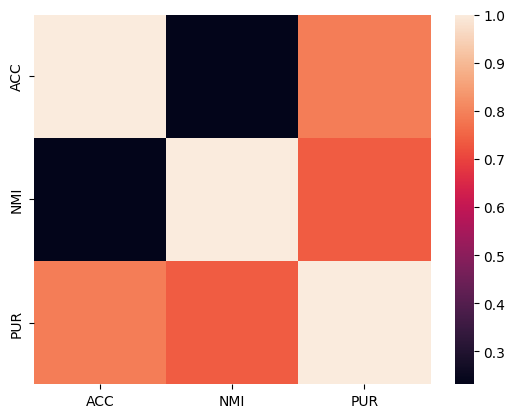
\includegraphics[width=\linewidth]{Images/cor_mcles.png}
     	   \caption{avec MCLES}
     	   \label{fig:bagmcles_cor}
     	   \end{subfigure}
        \begin{subfigure}{0.4\linewidth}
     	   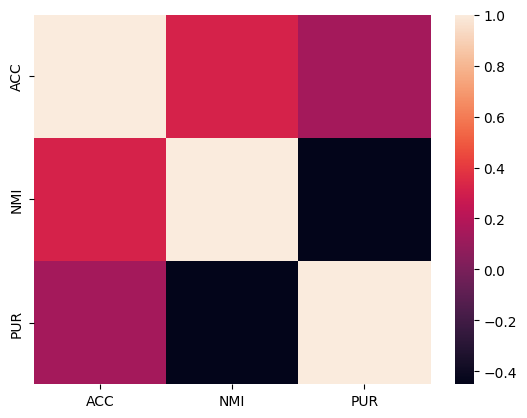
\includegraphics[width=\linewidth]{Images/cor_mvgl.png}
     	   \caption{avec MVGL}
     	   \label{fig:bagmvgl_cor}
        \end{subfigure}
        \caption{Corrélations entre métriques pour la méthode de type Bagging}
        \label{fig:bag_cor}
    \end{figure}

    Ces valeurs de paramètres visibles au Tableau \ref{table:default} ont été utilisées pour la réalisation des expérimentations dont les résultats sont sur le Tableau \ref{table:perfs}.
    %Ce tableau nous permet de tirer les conclusions suivantes:
	%\begin{itemize}
	%	\item Les modèles d'apprentissage ensemblistes sont plus performants que les modèles de base généralement
	%	\item Si les weak-learners sont stables, le modèle d'ensemble les exploitant le sera moins
	%	\item Si plutôt ils sont instables, le modèle d'ensemble les utilisant le sera plus
	%\end{itemize}
    %Cela peut se justifier car \acrshort{MVGL} s'assure de l'existence des composantes connexes correspondantes aux clusters voulus et \acrshort{MCLES} utilise l'algorithme KMEANS pour construire les clusters (ce qui le rend moins stable).
    %De plus, toutes ces observations nous montrent que MVGL a une grande variance que MCLES principalement au vue du nombre de weak-learners utilisés.
    
	\begin{table}[h!]
  	  \caption{Tableau de comparaison des performances}
  	  \centering
  		  \begin{tabular}{lrrr}
  		  \toprule
   		  & ACC & NMI & PUR \\
  		  model &  &  &  \\
  		  \midrule
  		  MVGL & 0.600$\pm$0 & 0.595$\pm$0 & 0.657$\pm$0 \\
  		  Bagging avec MVGL & \textbf{0.615$\pm$0.036} & \textbf{0.643$\pm$0.029} & \textbf{0.623$\pm$0.020} \\
  		  MCLES & 0.720$\pm$0.058 & 0.718$\pm$0.033 & 0.755$\pm$0.047 \\
  		  Bagging avec MCLES & \textbf{0.801$\pm$0.022}& \textbf{0.743$\pm$0.014} & \textbf{0.811$\pm$0.014} \\
  		  \bottomrule
  		  \end{tabular}
  	  \label{table:perfs}
	\end{table}
    
	%De ce fait on peut émettre l'hypothèse qu'orienter la construction des échantillons vers des exemples mal groupés pourrait augmenter les performances, car permettrait d'apprendre des structures complexes dans les données, qui empêchent la construction de meilleures clusters.
    %Ce qui pourrait amener à se poser la question de l'importance de chacune des vues dans la construction des clusters, au vue de leurs qualités.
